% !TEX spellcheck = en_US

% !TEX root = elastophi-report.tex


\section{Results}

%\begin{figure}[p]
%\centering
%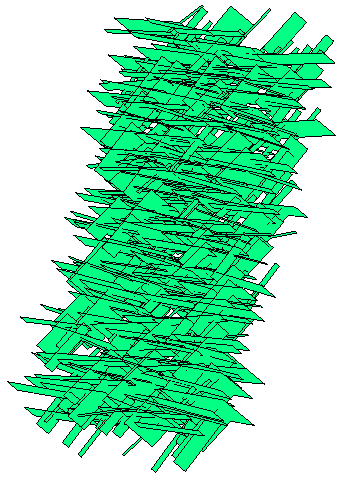
\includegraphics[width=0.4\textwidth]{../images/visu_maillage450Fracs.png}
%\caption{maillage450Fracs}
%\label{fig:maillage450Fracs}
%\end{figure}


\begin{figure}[p]
\centering
\subfloat[][Mesh.]
   {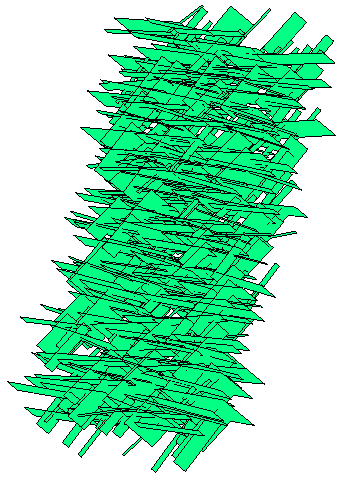
\includegraphics[width=.3\textwidth]{../images/visu_maillage450Fracs.png}} \quad
\subfloat[][Matrix compression for $\eta=1, \varepsilon=0.9$.]
   {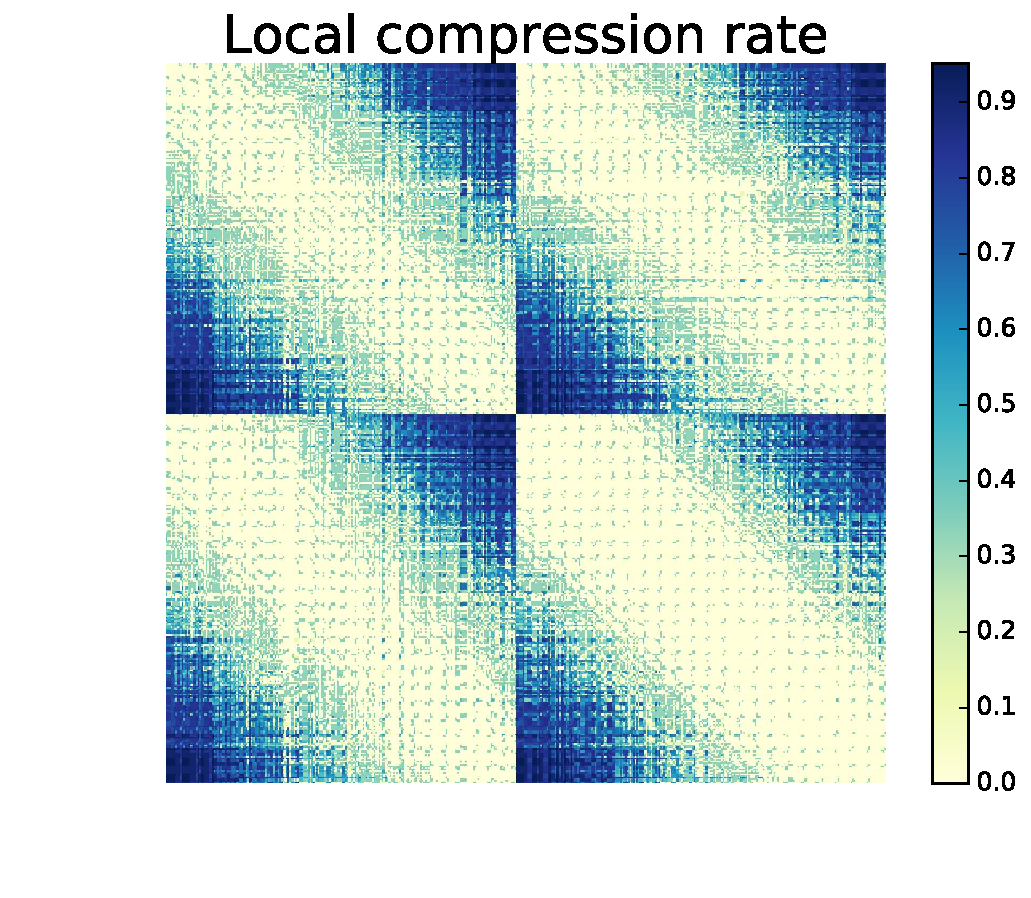
\includegraphics[width=.4\textwidth]{../images/graphe_mapp_output_local_comp_1_0,9_matrice450Fracs.pdf}} \\
\subfloat[][Matrix compression for $\eta=10, \varepsilon=0.9$.]
   {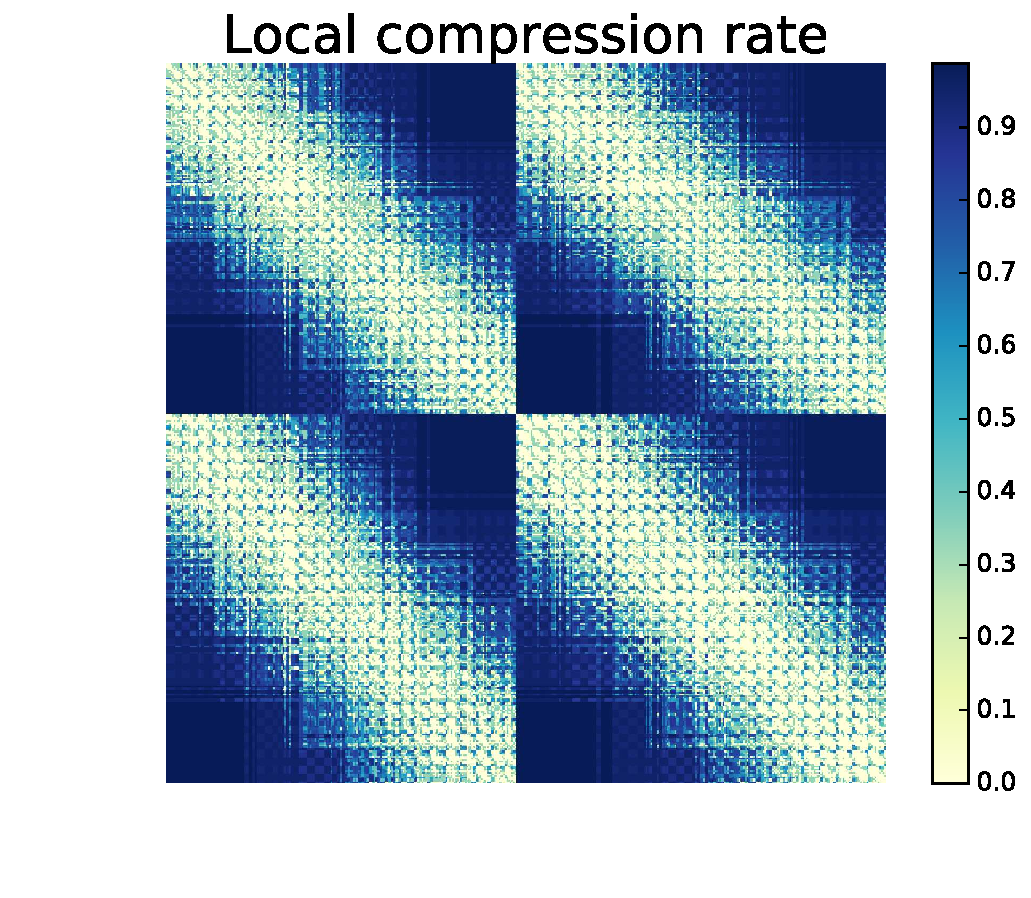
\includegraphics[width=.4\textwidth]{../images/graphe_mapp_output_local_comp_10_0,9_matrice450Fracs.pdf}}
\subfloat[][Matrix compression for $\eta=10, \varepsilon=1$.]
   {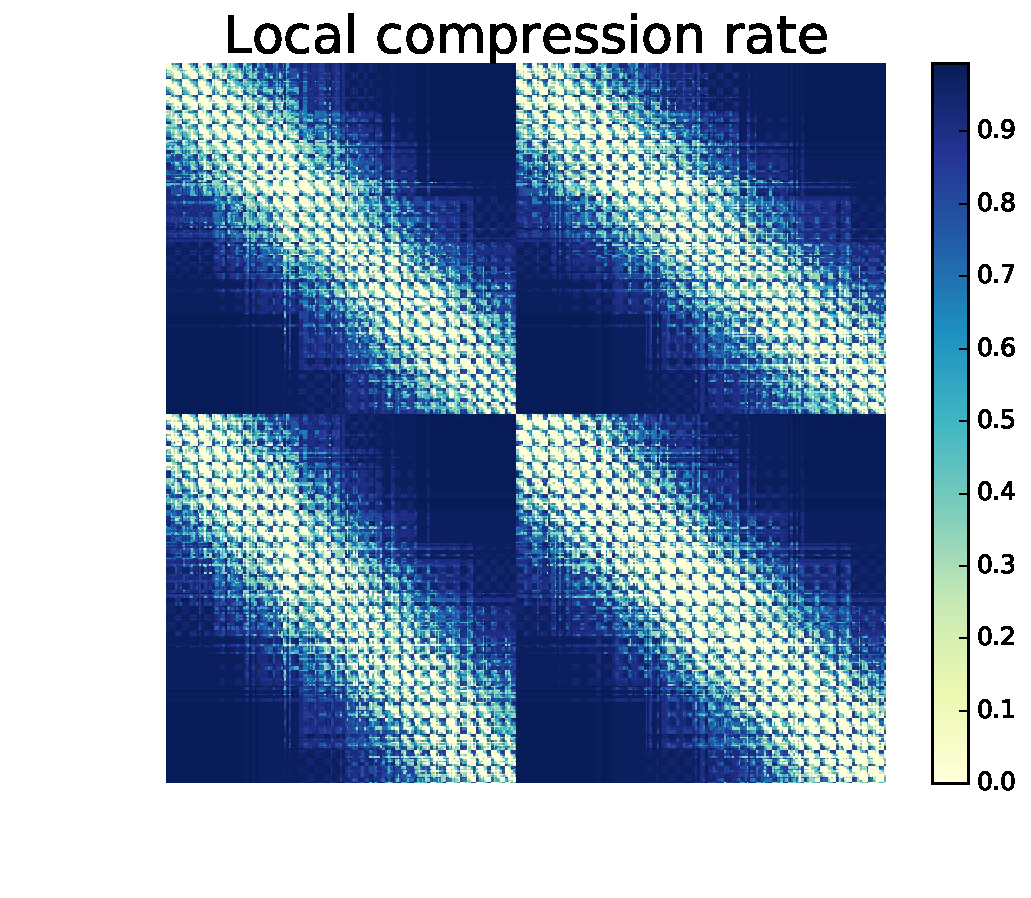
\includegraphics[width=.4\textwidth]{../images/graphe_mapp_output_local_comp_10_1_matrice450Fracs.pdf}} \\
\subfloat[][Errors and compression rates for different values of $\eta$ and $\varepsilon$.]
   {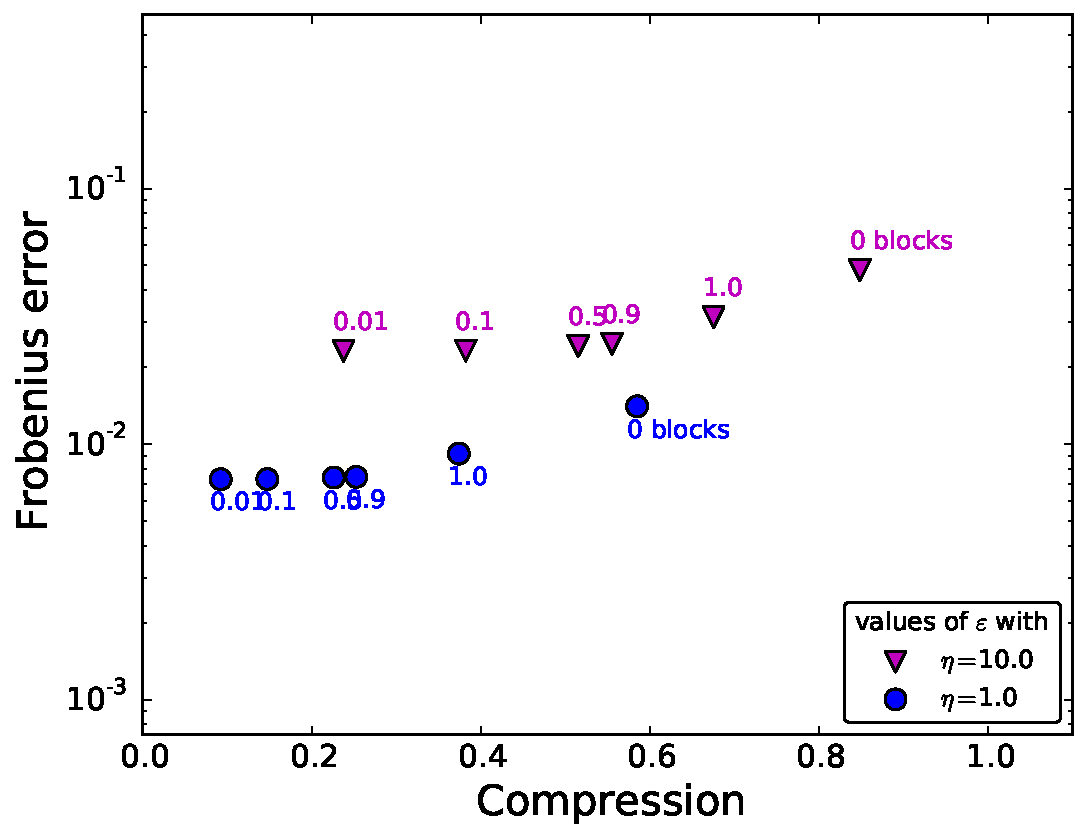
\includegraphics[width=.6\textwidth]{../images/graphe_compare_output_compression_18_08_2016matrice450Fracs.pdf}}
\caption{Results for the structure with $450$ fractures.}
\label{fig:subfig}
\end{figure}

\begin{figure}[p]
\centering
\subfloat[][Mesh.]
   {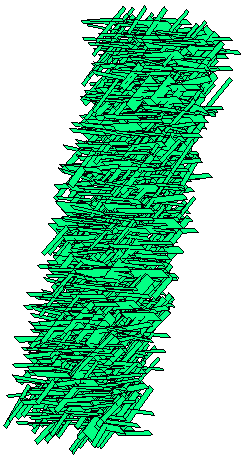
\includegraphics[width=.3\textwidth]{../images/visu_maillage1363Fracs.png}} \quad
\subfloat[][Matrix compression for $\eta=1, \varepsilon=0.9$.]
   {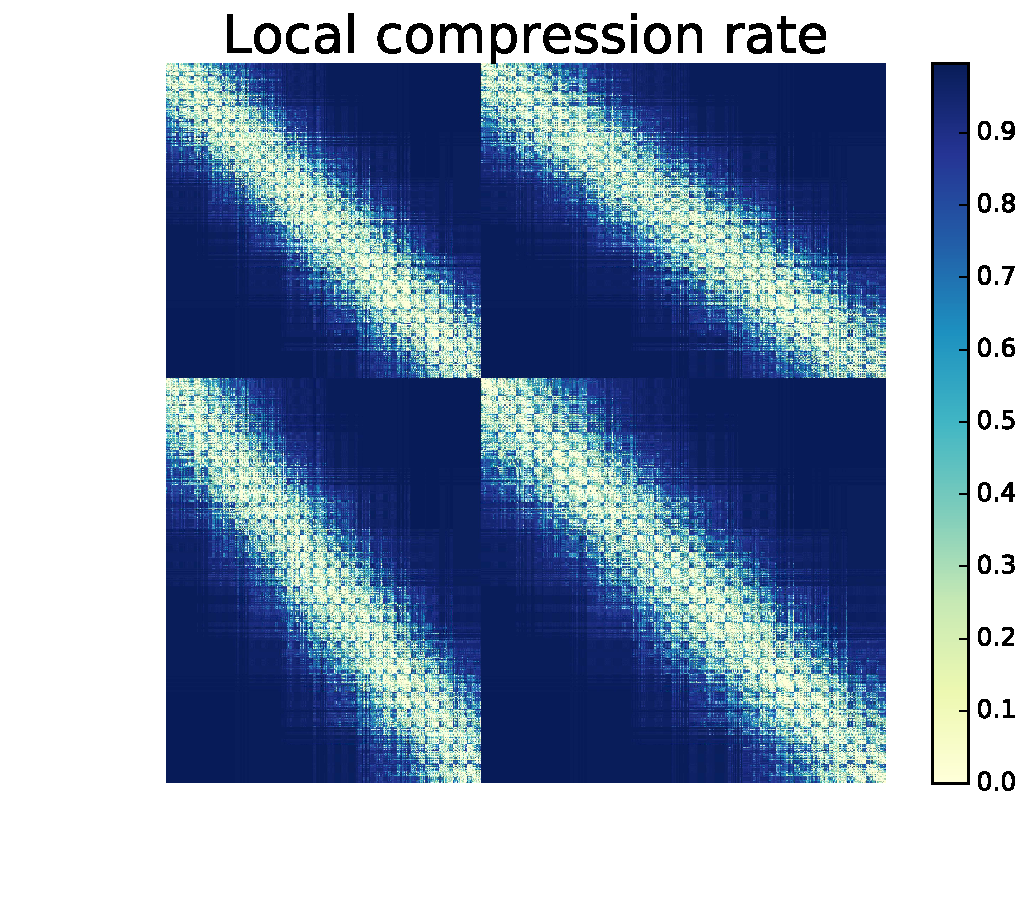
\includegraphics[width=.4\textwidth]{../images/graphe_mapp_output_local_comp_10_0,9_matrice1363Fracs.pdf}}\\
\subfloat[][Errors and compression rates for different values of $\eta$ and $\varepsilon$.]
   {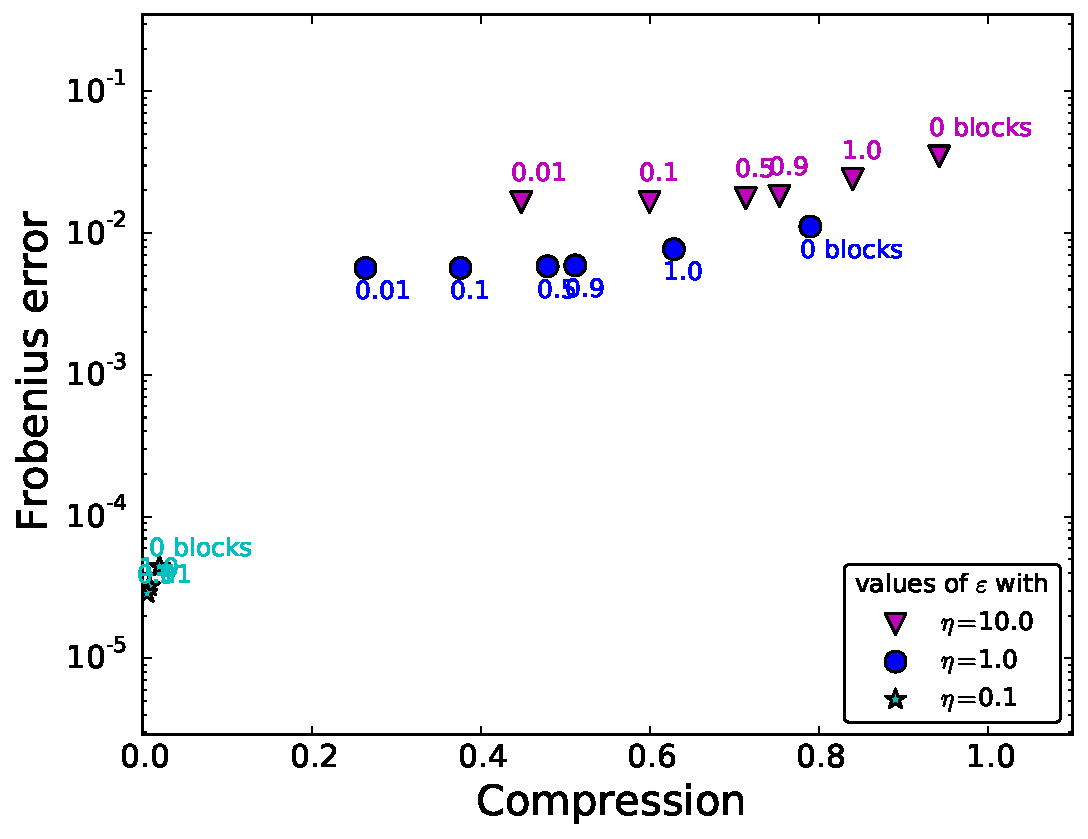
\includegraphics[width=.6\textwidth]{../images/graphe_compare_output_compression_18_08_2016matrice1363Fracs.pdf}}
\caption{Results for the structure with $1363$ fractures.}
\label{fig:subfig}
\end{figure}

\begin{figure}[p]
\centering
\subfloat[][Mesh.]
   {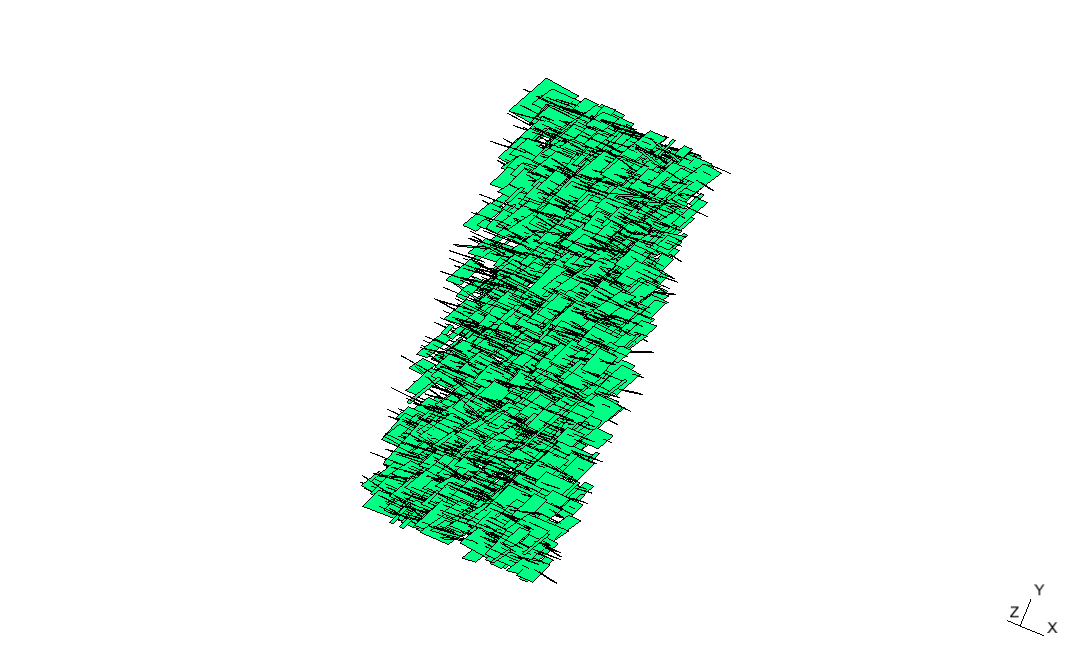
\includegraphics[width=.35\textwidth]{../images/visu_maillage1994Fracs.png}} 
\subfloat[][Errors and compression rates for different values of $\eta$ and $\varepsilon$.]
   {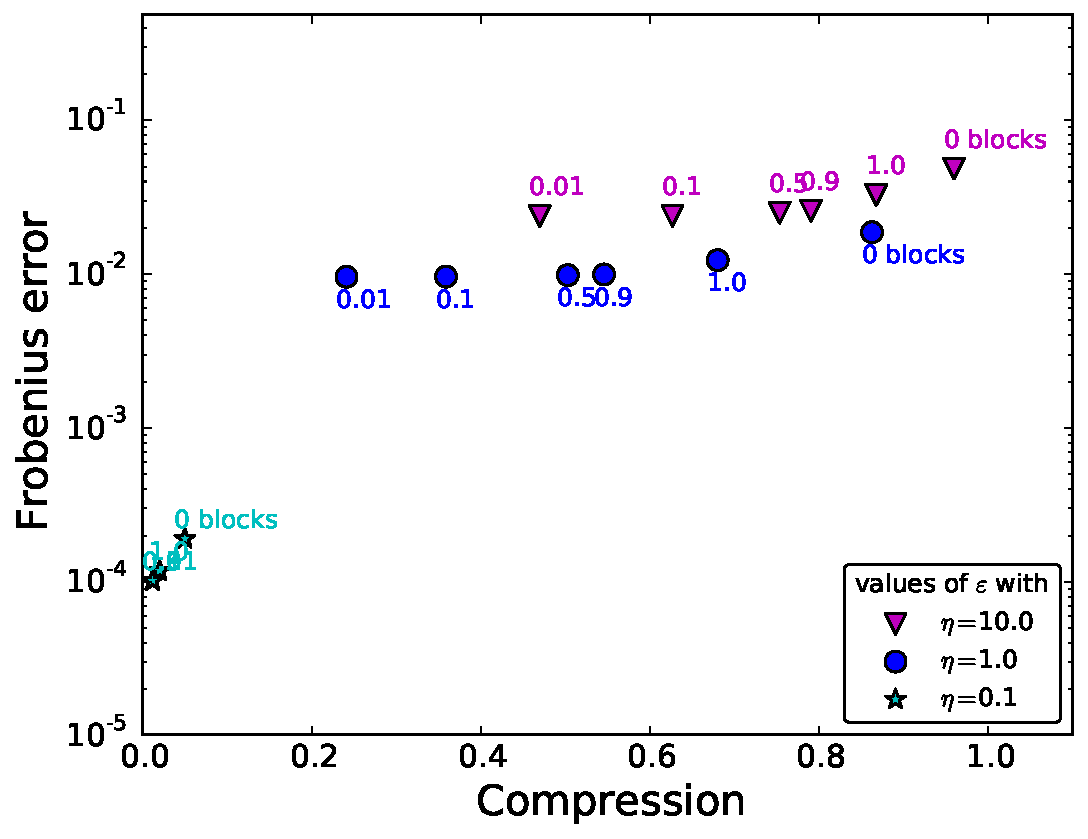
\includegraphics[width=.6\textwidth]{../images/graphe_compare_output_compression_18_08_2016matrice1994Fracs.pdf}}\\
\subfloat[][Times to build the HM-ACA matrix and compression rates for different values of $\eta$ and $\varepsilon$.]
   {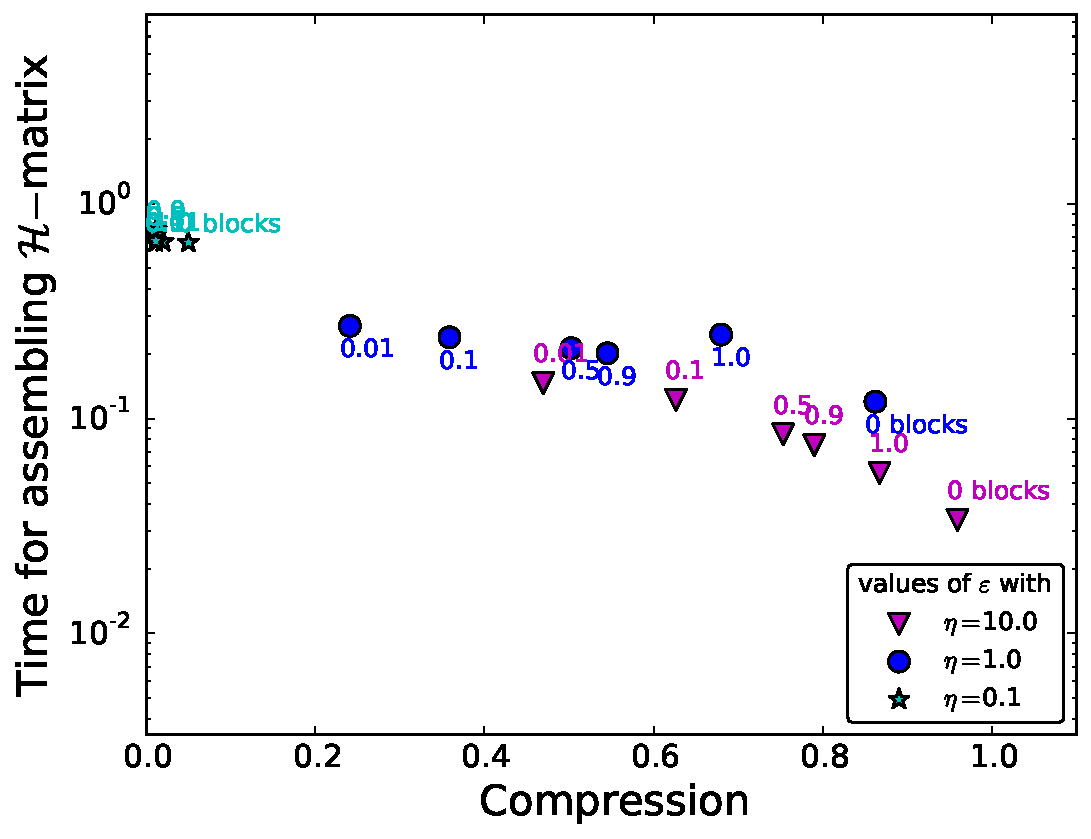
\includegraphics[width=.46\textwidth]{../images/graphe_tas_output_compression_18_08_2016matrice1994Fracs.pdf}} \;
\subfloat[][Times to build the HM-ACA matrix and compression rates for different values of $\eta$ and $\varepsilon$.]
   {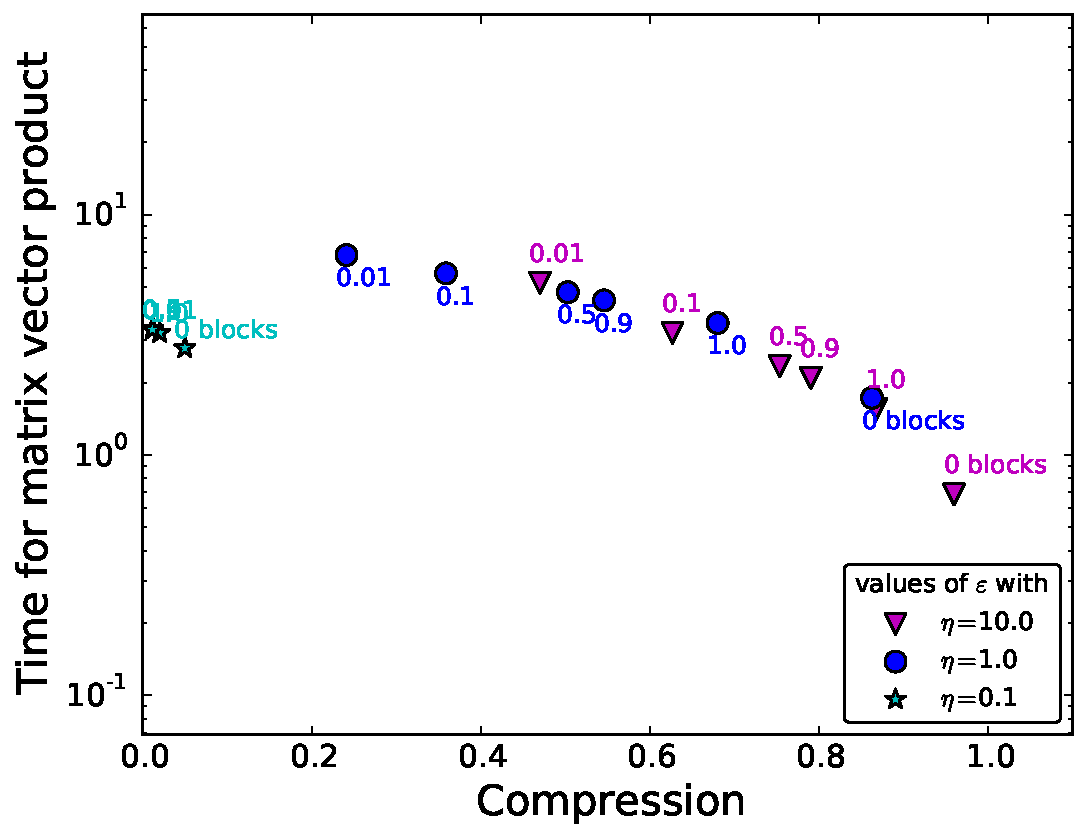
\includegraphics[width=.46\textwidth]{../images/graphe_tmv_output_compression_18_08_2016matrice1994Fracs.pdf}}
\caption{Results for the structure with $1994$ fractures.}
\label{fig:subfig}
\end{figure}

\begin{figure}[p]
\centering
\subfloat[][Mesh.]
   {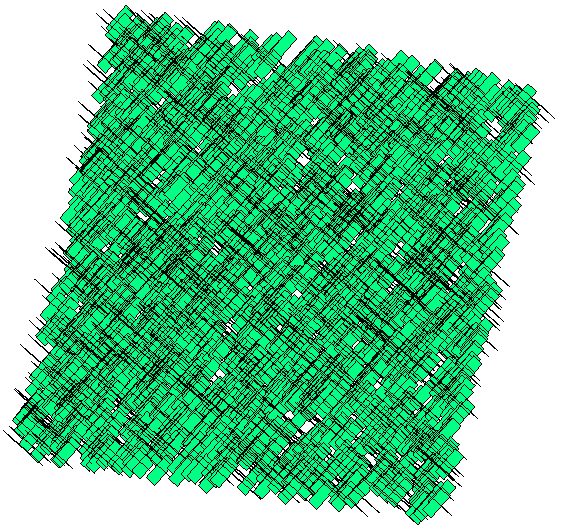
\includegraphics[width=.21\textwidth]{../images/visu_maillage2700FracsV1D1.png}} \qquad
\subfloat[][Errors and compression rates.] %for different values of $\eta$ and $\varepsilon$.]
   {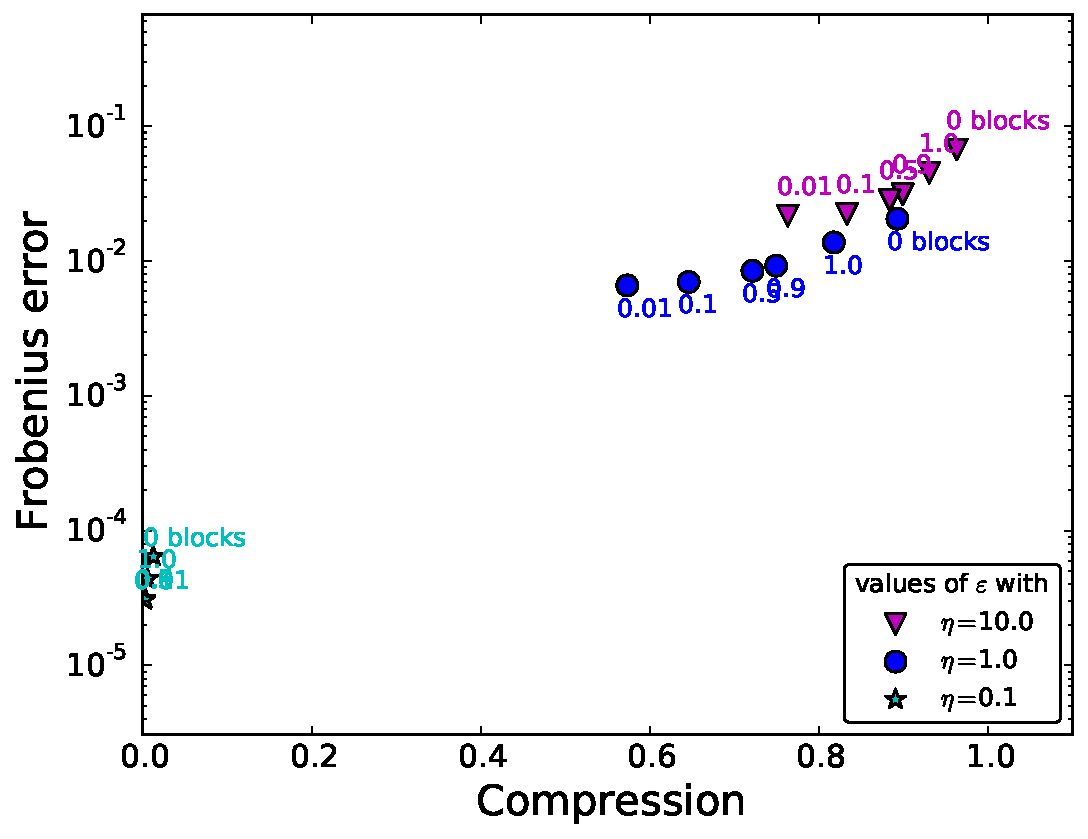
\includegraphics[width=.46\textwidth]{../images/graphe_compare_output_compression_18_08_2016matrice2700FracsV1D1.pdf}}
\caption{Results for the structure with $2700$ fractures inside a volume $V_1=300\times300\times20$.}
\label{fig:subfig}
\end{figure}

\begin{figure}[p]
\centering
\subfloat[][Mesh.]
   {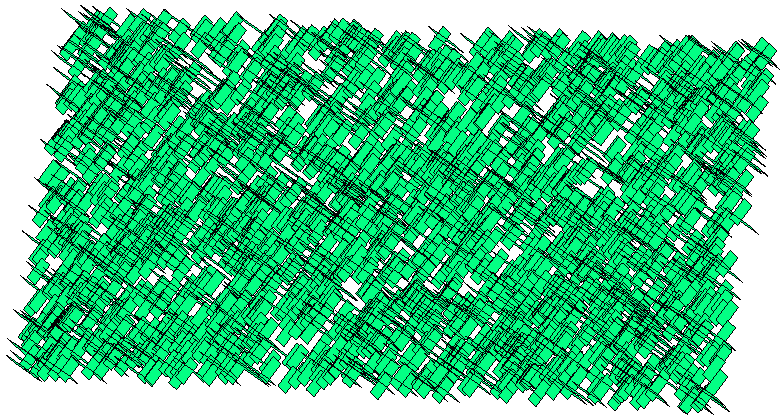
\includegraphics[width=.36\textwidth]{../images/visu_maillage2700FracsV2D2.png}} \qquad
\subfloat[][Errors and compression rates.] %for different values of $\eta$ and $\varepsilon$.]
   {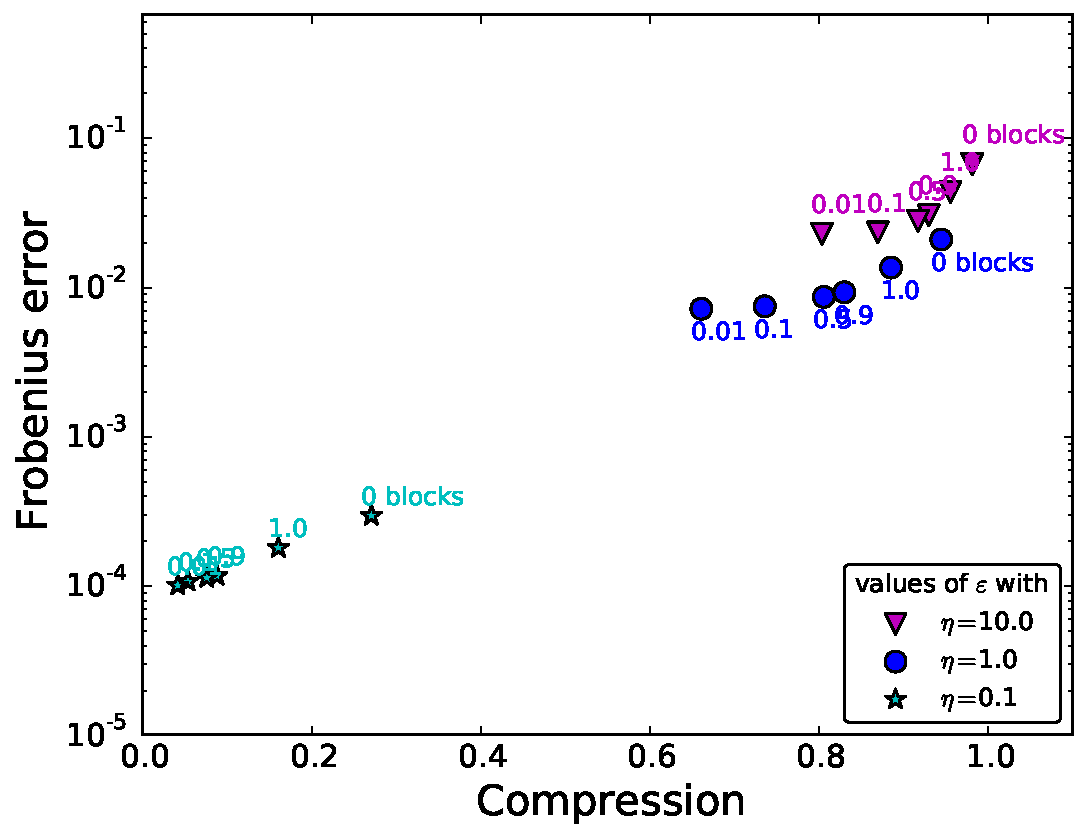
\includegraphics[width=.46\textwidth]{../images/graphe_compare_output_compression_18_08_2016matrice2700FracsV2D2.pdf}}
\caption{Results for the structure with $2700$ fractures inside a volume $V_2=600\times300\times20$.}
\label{fig:subfig}
\end{figure}

\begin{figure}[p]
\centering
\subfloat[][Mesh.]
   {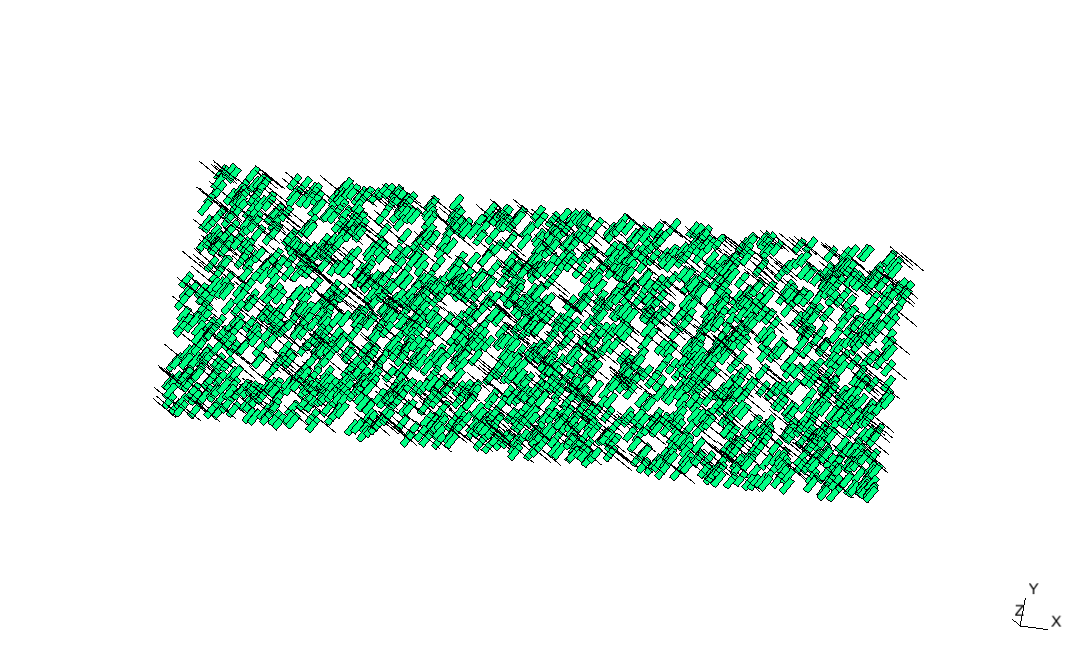
\includegraphics[width=.539\textwidth]{../images/visu_maillage2700FracsV3D3.png}}
\subfloat[][Errors and compression rates.] %for different values of $\eta$ and $\varepsilon$.]
   {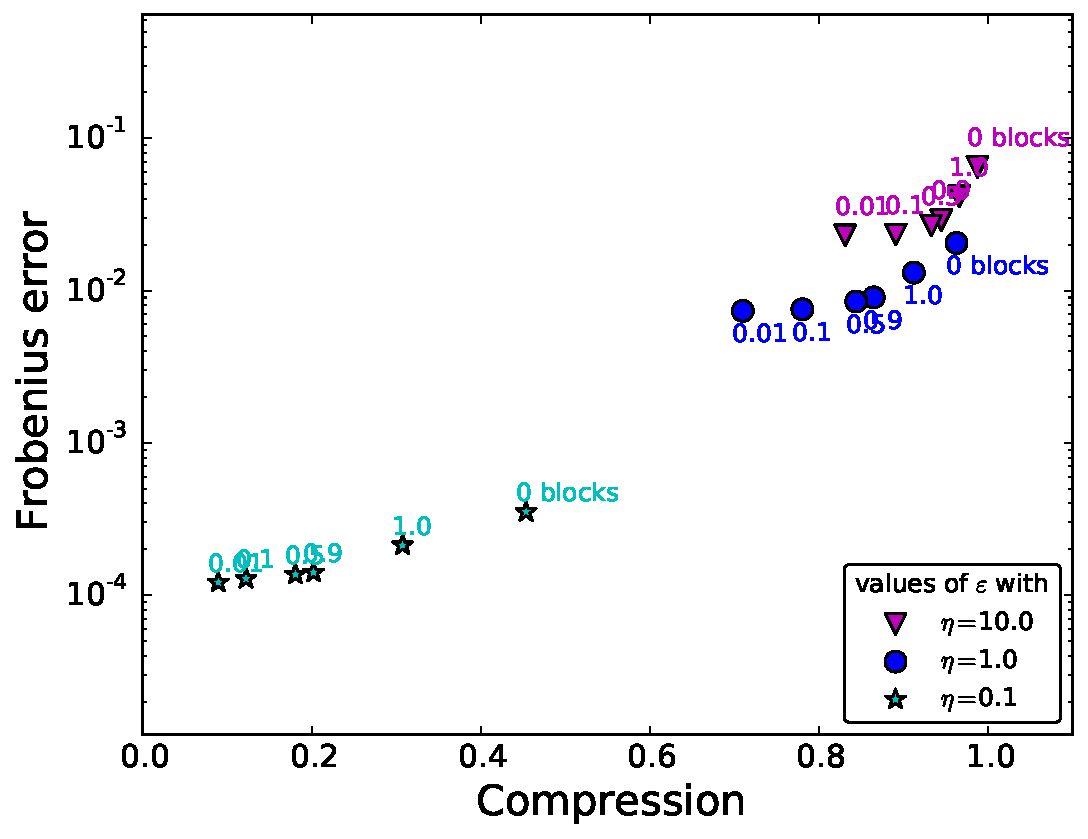
\includegraphics[width=.46\textwidth]{../images/graphe_compare_output_compression_18_08_2016matrice2700FracsV3D3.pdf}}
\caption{Results for the structure with $2700$ fractures inside a volume $V_3=900\times300\times20$.}
\label{fig:subfig}
\end{figure}

%$V_2=600\times300\times20$
%$V_3=900\times300\times20$

